\section{Side Channels in Interconnects}
\label{sec:interconnect-sc-bg}
Conceptually, carrying out a side-channel interconnect is very similar to carrying out such an attack on internet networks. 
The attacker creates congestion on a buffer in the communication path between the host (CPU) and the peripheral (e.g. GPU) and observes their own delay.
This delay would be proportional to the amount of data transferred by the victim, which would help the attacker gain insight into the victim's traffic shape.

However, a few differences between interconnects and traditional networks make it challenging to implement such an attack. \\
\textit{First}, The bandwidth of interconnects like PCIe is at least an order of magnitude higher than that of internet networks.
While a typical bandwidth in an internet network may be 1-10Gbps ( = 0.125 - 1.25 GBps), PCIe 4.0 can operate at a rate of 32GBps.
The high bandwidth makes it non-trivial to saturate the PCIe link. \\
\textit{Second}, latency in PCIe is at least three orders of magnitude smaller than that of internet networks.
Typically, internet latency is measured in milliseconds, while PCIe latency is measured in microseconds.
The low latency makes it difficult for the attacker to measure the delays accurately. \\
\textit{Third}, unlike internet networks, PCIe does not extend outside the machine of the host CPU.
This further adds to the challenge that the attacker needs to co-locate with the victim application on the same machine. \\
\textit{Fourth}, the PCIe protocol has a fixed behaviour depending on the type of transaction. 
Most transaction types can not generate enough traffic to even come close to saturating the bandwidth of PCIe. 
While saturating the bandwidth may not be necessary to create a side-channel attack, it would be useful if there is always at least one attacker packet in the buffer whenever the victim might transmit.
This would ensure that the attacker can observe a delay in their own packets for each packet or set of packets the victim transmits.

We provide a list of the transactions PCIe supports in \Cref{tab:pcie-transaction-types}, and a description of what each PCIe transaction type entails below: \\
\textbf{Posted:} Transactions where no response is issued or expected. 
These transactions are also asynchronous and hence allow multiple transactions of the same type to be in flight at the same time.\\
\textbf{Non-posted:} Transactions where a response is required. 
These types of transactions are also synchronous.
As such, one can not execute multiple of these simultaneously.\\
\textbf{Completions:} The completion of a previous non-posted transaction.\\

\begin{table}[h]
    \centering
    \begin{tabular}{|l|l|p{0.65\textwidth}|}
        \hline
        \textbf{Transaction} & \textbf{Type} & \textbf{Description} \\ 
        \hline
        Memory Read         & Non-Posted & Read from a memory-mapped address space \\ 
        Memory Write        & Posted     & Write to a memory-mapped address space  \\ 
        I/O Read            & Non-Posted & (Legacy PCI) Read from the I/O address space \\ 
        I/O Write           & Non-Posted & (Legacy PCI) Write to the I/O address space \\ 
        Configuration Read  & Non-Posted & Read control and status registers of the PCIe interface \\ 
        Configuration Write & Non-Posted & Write control and status registers of the PCIe interface \\  
        Message             & Posted     & Conveys information that isn't an access to an addressable space (e.g. Interrupts, Power Management, Error Signalling, Vendor-defined messaging). \\
        Completion          & Completion & Response to all non-posted transactions \\ 
        \hline
    \end{tabular}
    \caption{PCIe transaction types}
    \label{tab:pcie-transaction-types}
\end{table}


\subsection{Challenge: Measuring the time of PCIe transactions}

In \Cref{tab:pcie-transaction-types}, we can see that most PCIe transactions are Non-posted.
Only memory writes and messages are posted and hence asynchronous.
Asynchronous transactions such as a memory write (i.e. a \textit{store} instruction executed on memory-mapped PCIe endpoint memory region) would be more useful for carrying out a side-channel attack on PCIe.
This is because asynchronous transactions enable the attacker to have one transaction always pending to be sent out, regardless of the completion of the previous transaction(s).

However, measuring the completion time of an individual asynchronous transaction becomes more challenging as they are executed out-of-order. 
The naive solution of having a memory fence after each \textit{store} instruction would not work, as the memory fence would not allow the next \textit{store} instruction to be issued in parallel to the previous one, negating the benefit of using an asynchronous transaction.

\section{AMD CPU Architecture}
\label{subsec:amd-arch-bg}

Modern CPUs consist of many components, such as execution units, caches, PCIe root complex, and DRAM controllers.
Some subset of these components is always traversed when data is sent to or from the CPU to the PCIe endpoints.
The behaviour of each individual component may impact how the side-channel attack is carried out.
As such, it becomes necessary to understand all the components that may be involved in a PCIe transaction.

\begin{figure}[!htb]
    \centering
    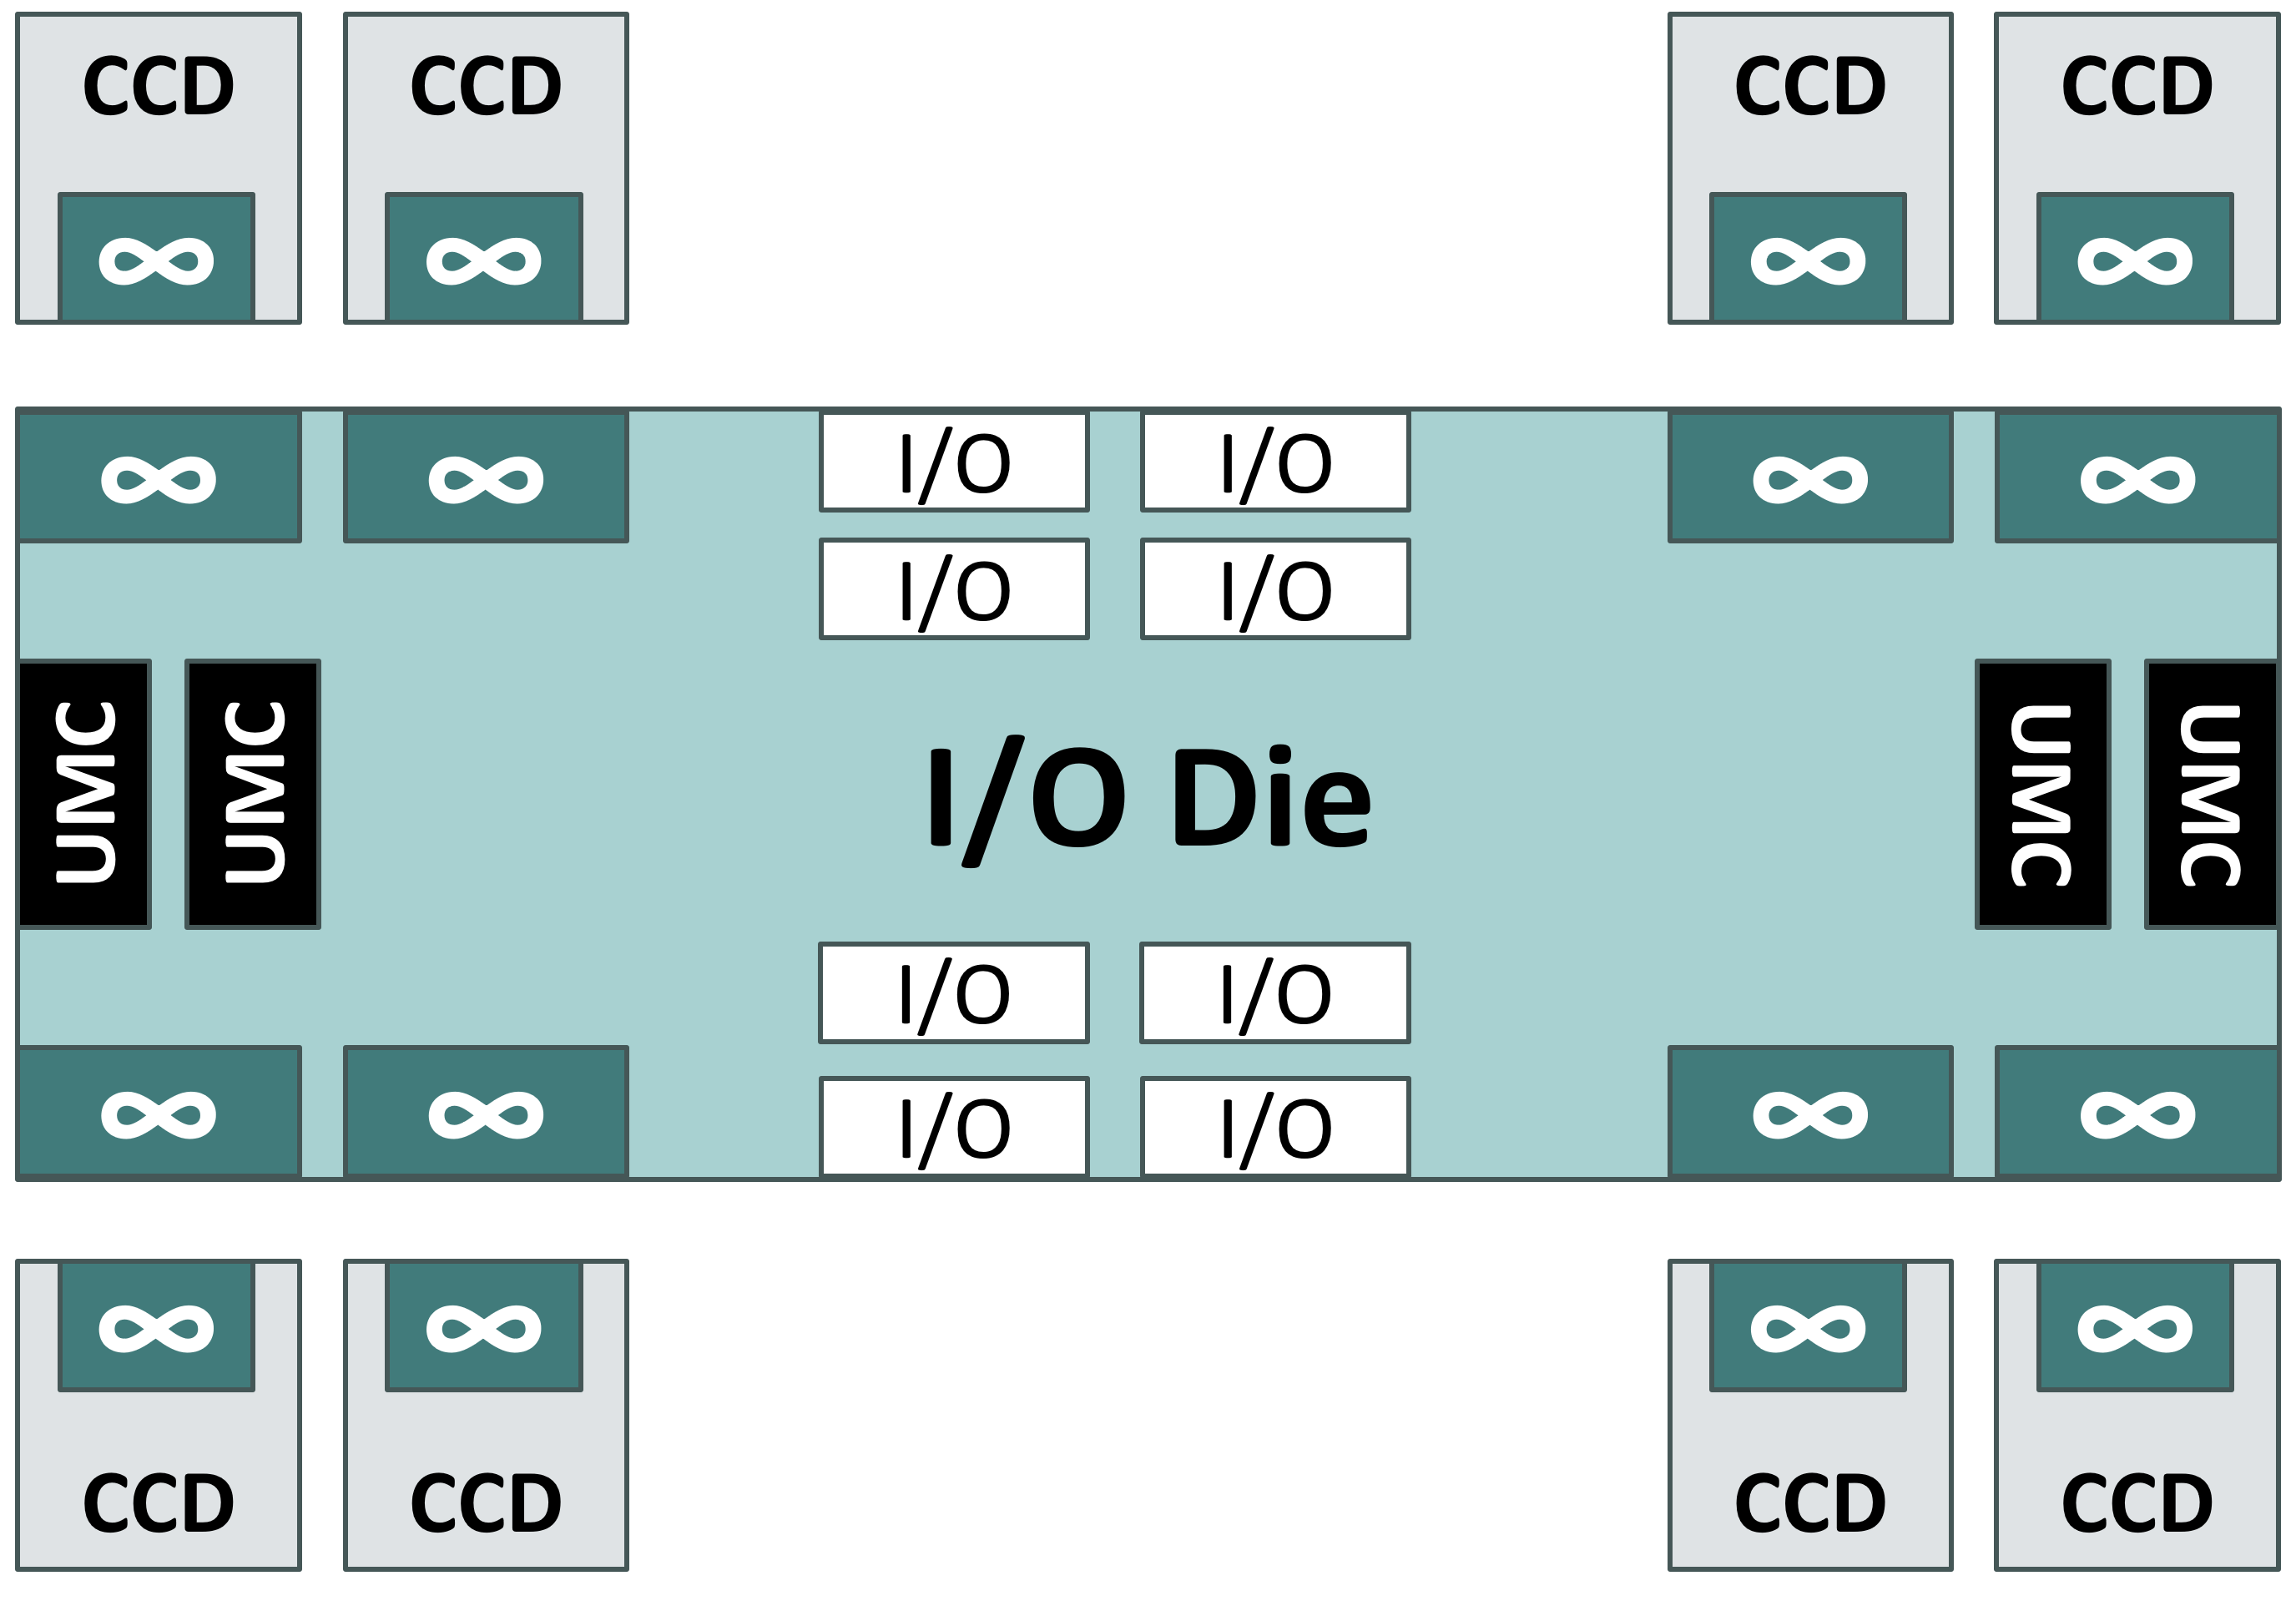
\includegraphics[width=\columnwidth]{figures/background/amd_arch/processor.png}
    \caption{AMD EPYC Zen 3 Architecture - CPU}
    \label{fig:amd-cpu}
\end{figure}


\Cref{fig:amd-cpu} shows a high-level overview of the architecture of the AMD EPYC Zen 3 processors.
The figure shows the following components:
\textbf{1) I/O:} The component that handles the input-output from the peripheral devices. This is where the PCIe communication happens.
\textbf{2) UMC:} The Unified Memory Controller is the controller that communicates with the DRAM.
\textbf{3) CCD:} The Core Complex Dies are where the cores (execution units) and caches reside.
\textbf{4) Infinity Fabric ($\infty$):} The interconnect that connects all of the components within the AMD CPU.

\subsubsection{CPU Pipelines}
\label{subsubsec:cpu-pipelines-bg}

Modern CPUs rely on executing multiple instructions simultaneously to maximise performance.
To achieve this, the CPUs have a multi-stage pipeline with the following stages: 1) Fetch, 2) Decode, 3) Schedule and Execute and 4) Retire.
We provide a simplified view of the pipeline in the CPU cores of the AMD EPYC Zen 3 processors in \Cref{fig:amd-core} and a brief description of each of the stages below:\\
\textbf{Fetch: } This stage fetches the next macro-op from the cache or the memory. 
However, the next macro-op to be fetched may not be deterministic, given the program may contain branches. 
In such cases, this stage also uses branch prediction to speculate on which instruction may be executed next and fetch that instruction.\\
\textbf{Decode: } This stage involved decoding the fetched macro-op into one or more micro-ops, which are then forwarded to the next stages.\\
\textbf{Schedule and Execute: } The scheduler(s) determine which instruction can be executed next based on the availability of the data that the instruction requires. 
This ensures that a long-running instruction (e.g., where the data is unavailable) does not stall all other independent instructions that can be executed.
As such, instructions here can be executed out of program order. 
Once the instruction has finished execution and the output of the instruction (if any) is available in the registers, the instruction is removed from the scheduler. 
\footnote{On AMD Zen 3 architecture, each scheduler has a capacity of 24 entries.}
As load and store are common but time-consuming instructions, this stage also consists of a load-store queue where pending load and store operations are held. \\
\textbf{Retire: } This stage ensures that instructions are retired in the program order so that the program can remain oblivious to the out-of-order execution that occurred in the previous stage.

\begin{figure}[!htb]
    \centering
    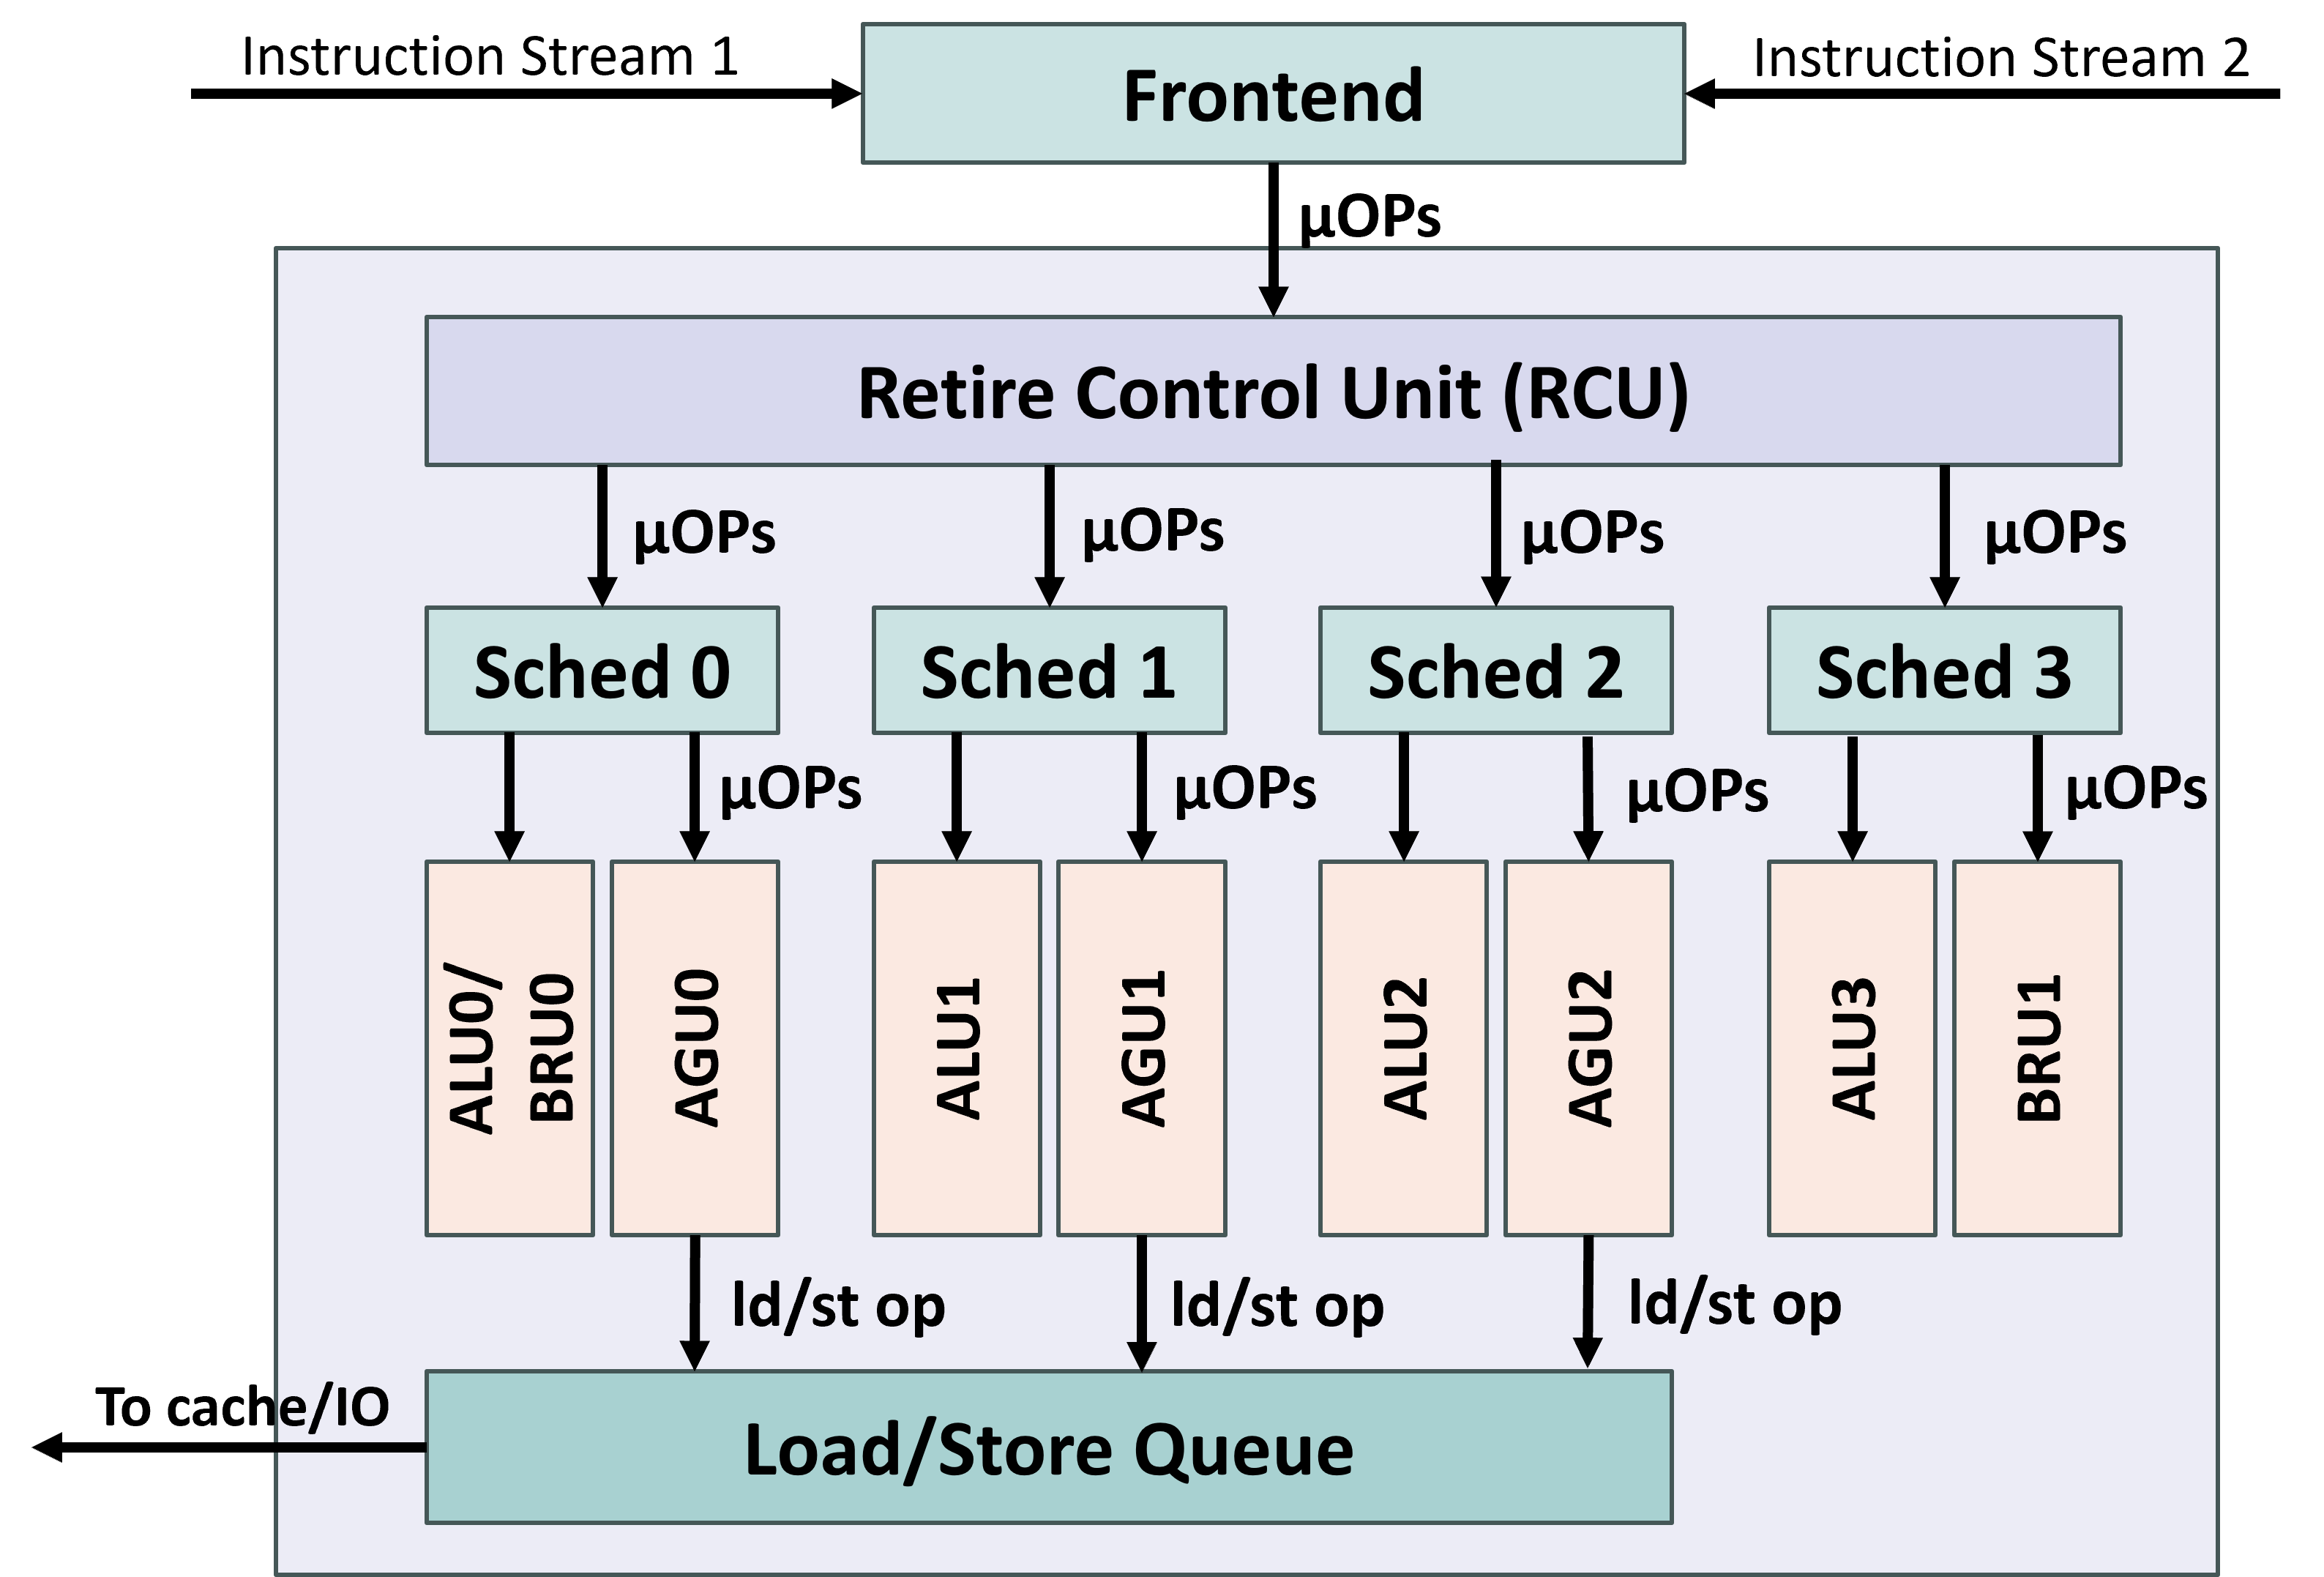
\includegraphics[width=\columnwidth]{figures/background/amd_arch/core.png}
    \caption{AMD EPYC Zen 3 Architecture - Core}
    \label{fig:amd-core}
\end{figure}

\subsubsection{PCIe transactions to/from CPU}

A program running on the CPU can transfer data to the PCIe device/endpoint in two major ways: 1) Memory operations via memory-mapped IO (MMIO) and 2) Direct memory access (DMA).
MMIO enables the CPU to map some memory region of the PCIe endpoint in the CPU's physical address space.
Any process with the proper permissions can then map this memory within the process and perform normal \textit{load} or \textit{store} operations on this memory.
However, this approach requires the execution units of the CPU to issue repeated \textit{load/store} instructions to copy data to the PCIe endpoint.
While this method is useful for reading or writing limited content, such as small configuration parameters, to the PCIe endpoints, it is inefficient for transferring a large amount of data.
To alleviate this, a lot of PCIe endpoints consist of a special hardware component called a DMA engine.
The DMA engine can copy large chunks of contiguous data without involving the execution units of the CPU.

For MMIO-based transactions, the load or store instructions go through the same instruction pipeline outlined in \Cref{fig:amd-core}. 
From the Load Store Queue, they end up in the I/O die outlined in \Cref{fig:amd-cpu} and go out the I/O block to the connected PCIe endpoint.
For DMA transactions (usually initiated by the PCIe endpoint), the transaction comes into the I/O block and, after some address and protocol translations, is sent out to the DRAM via the UMC.

\endinput



\endinput




https://www.linkedin.com/pulse/pci-express-primer-3-transaction-layer-simon-southwell/